% ****** Start of file aipsamp.tex ******
%
%   This file is part of the AIP files in the AIP distribution for REVTeX 4.
%   Version 4.1 of REVTeX, October 2009
%
%   Copyright (c) 2009 American Institute of Physics.
%
%   See the AIP README file for restrictions and more information.
%
% TeX'ing this file requires that you have AMS-LaTeX 2.0 installed
% as well as the rest of the prerequisites for REVTeX 4.1
% 
% It also requires running BibTeX. The commands are as follows:
%
%  1)  latex  aipsamp
%  2)  bibtex aipsamp
%  3)  latex  aipsamp
%  4)  latex  aipsamp
%
% Use this file as a source of example code for your aip document.
% Use the file aiptemplate.tex as a template for your document.
%\documentclass[aps,prl,twocolumn,showpacs,superscriptaddress]{revtex4-1}
\documentclass[%
 aip,
 floatfix,
% jmp,
% bmf,
% sd,
% rsi,
 amsmath,amssymb,
%preprint,%
 reprint,%
%author-year,%
%author-numerical,%
% Conference Proceedings
]{revtex4-1}


 
% \usepackage[justification=justified,
%   format=plain]{subcaption}
% \usepackage[justification=justified,
%   format=plain]{caption}
\usepackage{subfigure}
\usepackage{graphicx}% Include figure files




\usepackage{dcolumn}% Align table columns on decimal point
\usepackage{bm}% bold math
%\usepackage[mathlines]{lineno}% Enable numbering of text and display math
%\linenumbers\relax % Commence numbering lines

\usepackage[utf8]{inputenc}
\usepackage[T1]{fontenc}
\usepackage{mathptmx}
\usepackage{etoolbox}
\usepackage{amsmath}
\usepackage{pbox}

\newcommand{\id}{\mathbf{1}}
\newcommand{\ri}{\mathrm{i}}
\newcommand{\re}{{\mathrm e}}
\newcommand{\rd}{\mathrm{d}}
\newcommand{\rs}{\mathrm{s}}
\newcommand{\rb}{\mathrm{b}}
\newcommand{\rJ}{\mathrm{J}}
\newcommand{\Jb}{\mathcal{J}}
\newcommand{\no}{\hat{n}}
%\renewcommand{\ao}{\hat{a}}
\renewcommand{\aa}{\hat{a}^\dag}
\newcommand{\Ho}{H}%{\hat{H}}
\newcommand{\Uo}{U}%{\hat{U}}
\newcommand{\Vo}{\hat{V}}
\newcommand{\Fo}{\hat{F}}
\newcommand{\Ko}{\hat{K}}
\newcommand{\Qo}{\hat{Q}}
\newcommand{\la}{\langle}
\newcommand{\ra}{\rangle}
\newcommand{\lla}{\langle\!\langle}
\newcommand{\rra}{\rangle\!\rangle}
\newcommand{\tr}{\mathrm{tr}}
\newcommand{\bn}{{\bm n}}
\newcommand{\bA}{{\bm A}}
\newcommand{\br}{{\bm r}}
\newcommand{\bro}{{\bm \rho}}
\newcommand{\bxi}{{\bm \xi}}
\newcommand{\bF}{{\bm F}}
\newcommand{\bp}{{\bm p}}
\newcommand{\ba}{{\bm a}}
\newcommand{\bk}{{\bm k}}
\newcommand{\bq}{{\bm q}}
\newcommand{\bx}{{\bm x}}
\newcommand{\be}{\begin{equation}}
\newcommand{\ee}{\end{equation}}
\newcommand{\bes}{\begin{eqnarray}}
\newcommand{\ees}{\end{eqnarray}}
\newcommand{\ket}[1]{{\left|  #1 \right\rangle}}
\newcommand{\kket}[1]{{\left|  #1 \right\rrangle}}
\newcommand{\bra}[1]{{\left\langle  #1 \right|}}
\newcommand{\bbra}[1]{{\left\llangle  #1 \right|}}
\newcommand{\braket}[2]{{\left\langle #1 \,| #2\right\rangle}}
\newcommand{\bbrakket}[2]{{\left\llangle #1 \,| #2\right\rrangle}}
\newcommand{\intd}[1]{{\int\!\mathrm{d} #1}}
\newcommand{\Ls}{\tilde\Lambda(s)}
\newcommand{\Lsinv}{\tilde\Lambda(s)^{-1}}
\newcommand{\Ks}{\tilde K(s)}
\renewcommand{\i}{\mathrm{i}}
\newcommand{\hide}[1]{{}}
%\DeclareMathOperator{\mod}{mod}
\newcommand{\cmt}[1]{{\color{red} \bf [#1]}}

\DeclareMathOperator{\arccot}{arccot}

%% Apr 2021: AIP requests that the corresponding 
%% email to be moved after the affiliations
\makeatletter
\def\@email#1#2{%
 \endgroup
 \patchcmd{\titleblock@produce}
  {\frontmatter@RRAPformat}
  {\frontmatter@RRAPformat{\produce@RRAP{*#1\href{mailto:#2}{#2}}}\frontmatter@RRAPformat}
  {}{}
}%
\makeatother

%%%%% COLORS
\usepackage{color,soul}
\definecolor{red}{rgb}{1,0,0}
\definecolor{green}{rgb}{0,0.6,0}
\definecolor{blue}{rgb}{0,0,1}
\newcommand{\sd}[1]{\textcolor{blue}{#1}}
\newcommand{\ss}[1]{\textcolor{green}{#1}}
\newcommand{\pl}[1]{\textcolor{red}{#1}}
\newcommand{\stpl}[1]{\setstcolor{red}{\st{#1}}} % overstriking
\newcommand{\stss}[1]{\setstcolor{green}{\st{#1}}} 
\newcommand{\stsd}[1]{\setstcolor{blue}{\st{#1}}} % overstriking

%%%%%%%%%%%%%%%%%%%%%%%%%%%%%%%%%%%%%%%%%%%%%%%
%%%%%%%%%%%%%%%%%%%%%%%%%%%%%%%%%%%%%%%%%%%%%%%
\begin{document}

\preprint{AIP/123-QED}

\title{Machine Learning for Digital Quantum Simulations: Do it with care 
}

\author{K.~Wold}
 \email{krisw@oslomet.no}
 \affiliation{Affiliation}

\author{S.~Denisov}
% \homepage{http://www.Second.institution.edu/~Charlie.Author.}
 %\email{sergiyde@oslomet.no}
 \affiliation{Department of Computer Science, Oslo Metropolitan University, Oslo N-0130 Oslo, Norway}
\affiliation{NordSTAR – Nordic Center for Sustainable and Trustworthy AI Research, Oslo N-0166, Norway}

\date{\today}

\begin{abstract}
Abstract
\end{abstract}

\maketitle

\begin{quotation}
Quotation
\end{quotation}

% Body of paper goes here. Use proper sectioning commands. 
% References should be done using the \cite, \ref, and \label commands

\section{Introduction\label{sec:1}}
Introduction

\section{Theory \label{sec:2}}

\subsection{Quantum Compiling}



Assume one wishes to execute some target quantum circuit $U_T$. This is not straight forward in practice, as real quantum hardware only implement a limited number of elementary quantum called the basis gates $\mathcal{G} = \{G_1, G_2, \cdots G_M\}$. Instead, one needs to compile $U_T$ into a sequence of gates $U_N = g_1 g_{2} \cdots g_N$, $g_i \in \mathcal{G}$, that approximates $U_T$ in the best possible way. Here, $N$ denotes the circuit depth of $U_N$. The Kitaev-Solovay theorem shows that some basis gates are universal, meaning that for any unitary $U_T$, there exists a finite sequence $U_N$ such that it approximates $U_T$ to arbitrary precision\cite{dawson2005solovaykitaev}. However, it is a highly non-trivial optimization problem to actually find this sequence. Furthermore, it should also be put emphasis on finding sequences as short as possible, since current quantum hardware is characterized by low coherence times.


When performing quantum compiling, one needs to decide upon a measure of similarity between the target circuit $U_T$ and the compiled circuit $U_N$. Here, there are two typical choices. If one wishes to approximate the complete effect of $U_T$, often called Full Unitary Matrix Compiling\cite{Khatri2019quantumassisted} (FUMC), a possible choice is the Average Gate Fidelity:

\begin{equation}\label{eq:AGFgeneral}
    \Bar{F}(U_T, U_N) = \int |\bra{\psi}U_T^{\dagger} U_N \ket{\psi}|^2 d\psi,
\end{equation}
where the integration is done with respect the whole Hilbert space of normalized wavefunctions $\psi$.  
In case we are working with a d-dimensional quantum system, i.e. $\ket{\psi} \in \mathbb{C}^{d}$ and $U_T, U_N \in \mathbb{C}^{d\times d}$, Eq. (\ref{eq:AGFgeneral}) simplifies to the form\cite{AGF}

\begin{equation}\label{eq:AGFfinite}
    \Bar{F}(U_T, U_N) = \frac{|\text{Tr}[U_T^{\dagger} U_N]|^2 + d^2}{d + d^2}.
\end{equation}

In case one wants to approximate the effect of $U_T$ only on a single input state $\ket{\psi_0}$, often called Fixed Input State Compiling\cite{Khatri2019quantumassisted} (FISC), one can measure the similarity in terms of the state fidelity

\begin{equation}\label{eq:state_fidelity}
    F(U_T, U_N, \psi_0) = |\bra{\psi_0}U_T^{\dagger} U_N\ket{\psi_0}|^2.
\end{equation}
For practical purposes, one can assume that the initial state is the all-zero state, i.e., $\ket{\psi_0} = \ket{\boldsymbol{0}}$. In this case, the state fidelity reduces to the Loschmidt Echo Test (LET) measure \cite{Goussev:2012}

\begin{equation}\label{eq:state_fidelity}
    F(U_T, U_N) = |\bra{\boldsymbol{0}}U_T^{\dagger} U_N\ket{\boldsymbol{0}}|^2.
\end{equation}
Eq. (\ref{eq:AGFfinite}) and Eq. (\ref{eq:state_fidelity}) have the property that $f(U_T, U_N) \in [0, 1]$, where $f$ is either of the aforementioned measures. Further, $f(U_T, U_N) = 1$ means that the circuits $U_T$ and $U_N$ have identical effects. Using this, it is typical to define the compilation as successful within a tolerance $\delta \in [0, 1]$ if
\begin{equation}
    f(U_T, U_N) > 1 - \delta.
\end{equation}

It is interesting to quantify the computational cost of quantum compiling in terms of how the compute time $t$ and circuit depth $N$ relate to the tolerance $\delta$. Both these quantities exhibit a polylogarithmic scaling relation with respect to the tolerance on the following form:


\begin{equation}\label{eq:scaling_relation}
    t,N \sim \mathcal{O}(\log^c(\delta^{-1})),
\end{equation}
for some positive power $c$. For lower  (stricter) tolerances $\delta$, more time and gates are required to obtain a sufficient approximation. \citet{HRC} showed, using a geometrical proof, that no compiling strategy could yield $c < 1$ for the scaling of circuit depth $N$. For one-qubit compiling, the Dawson-Nielsen algorithm \cite{dawson2005solovaykitaev}, based on the Solovay-Kitaev theorem, is able to compile circuits in time $\mathcal{O}(\log^{2.71}(\delta^{-1}))$ with depth $\mathcal{O}(\log^{3.97}(\delta^{-1}))$.


\subsection{Deep Reinforcement Learning}



\section{Methods\label{sec:3}}

\subsection{Basis Gates}
In this work we study the same one-qubit sets of basis gates as \citet{QCRL}. These are the Small-Rotations basis set \cite{QCRL} and the HRC basis set \cite{HRC}.

The former set of basis gates is defined as
\begin{equation}\label{eq:smallrotations1}
    \mathcal{G} = \bigg\{R_j\bigg (\pm\frac{\pi}{64}\bigg)|j\in\{x,y,z\}\bigg\},
\end{equation}
where $R_j(\theta)$ is the Pauli rotation operator around direction $j$ with angle $\theta$. 

The latter set of basis gates is defined by the operators
\begin{align}\label{eq:HRC1}
    V_1 = \frac{1}{\sqrt{5}}
          \begin{pmatrix}
          1 & 2i \\
          2i & 1 
          \end{pmatrix}\\
    V_2 = \frac{1}{\sqrt{5}}
          \begin{pmatrix}
          1 & 2 \\
          -2 & 1 
          \end{pmatrix}\\
    V_3 = \frac{1}{\sqrt{5}}
          \begin{pmatrix}
          1 +2i & 0 \\
          0 & 1 -2i 
          \end{pmatrix}
\end{align}
We also introduce natural extensions of these sets for two qubits in order to see how the various methods perform for larger systems. We define the two-qubit Small Rotations basis gates as single-qubit rotations on each qubit, together with the entangled rotations $R_{jj}(\pm) = \cos{(\pm \frac{\pi}{64})} I \otimes I - i \sin{(\pm \frac{\pi}{64})} J\otimes J$, where $J$ is one of the quantum gates $\{X, Y, Z\}$. This set can be summerized as
\begin{equation}\label{eq:smallrotations2}
    \mathcal{G} = \{R_j(\pm)\otimes I, I\otimes R_j(\pm), R_{jj}(\pm)  |j\in\{x,y,z\}\}.
\end{equation}
The HRC set extends to two qubits in much the same fashion by including the single-qubit HRC operators for both qubits. To introduce entanglement, we also include the $\sqrt{\text{SWAP}}$ gate (square root of swap gate). This gate is universal, meaning that any unitary can be constructed using only this gate and single qubit gates (kilde). The gate set can be summerized as 
\begin{equation}\label{eq:HRC2}
    \mathcal{G} = \{V_i\otimes I, I\otimes V_i    |i\in\{1,2,3\}\} \cup \{\sqrt{\text{SWAP}}\}.
\end{equation}
\subsection{Deep Reinforcement Learning for Quantum Compiling}

This section summarises and extends the work of \citet{QCRL} on deep reinforcement learning based quantum compiling.

Assume $U_n$, $n\leq N$, is the unitary containing the first $n$ gates of $U_N$. That is, it is a partially compiled circuit. \citet{QCRL} originally introduced the matrix quantity
\begin{equation}\label{eq:FUMCmetric}
    O_n = U_T^{\dagger}U_n,
\end{equation}
which serves as the features the neural policy is fed. The features are extracted by constructing a vector consisting of the real and imaginary parts of the elements of $O_n$ in the computational basis. We choose to call this quantity the discrepancy metric, as it encodes the complete information describing the discrepancy between $U_T$ and $U_n$. 

While the above expression is appropriate for FUMC, we introduce a discrepancy metric suitable for FISC:

\begin{equation}
    O_n = \bra{\boldsymbol{0}}U_T^{\dagger}U_n,
\end{equation}
which is a row vector in the computational basis.Note that if $U_n$ is a good approximation to $U_T$, we have that $O_n \approx I$ and $O_n \approx \bra{\boldsymbol{0}}$ up to a global phase for FUMC and FISC, respectivly.

A neural policy $\pi(O_n; \boldsymbol{\theta})$ (figure to come), parameterized by $\boldsymbol{\theta}$, predicts the next gate in the compiled sequence from $O_n$, i.e.,
\begin{align}
    a_{n+1} = \pi(O_n; \boldsymbol{\theta})\\
    g_{n+1} = G_{a_{n+1}},
\end{align}
where $g_i \in \mathcal{G} = \{G_1, \cdots, G_M\}$ is an elementary gate from the basis gate set. Hence, we get the recursive relationship
\begin{align}
    U_{n+1} = U_n g_{n+1}\\
    O_{n+1} = O_n g_{n+1},
\end{align}
which terminates after $N$ iterations, either when $f(U_T, U_N)> 1 - \delta$ and the compilations was successful, or when the number of gates reach a maximum amount $N=N_{max}$ and the compilation was unsuccessful. 

In this work, we utilize an agent with a neural policy based on $\epsilon$-greedy Q-learning (kilde). The policy can be formulated as
\begin{equation}\label{eq:policy}
    a_{n+1} = \pi(O_n; \boldsymbol{\theta}) =
    \begin{cases} 
        \underset{k}{\operatorname{argmax}} [Q(O_n, k; \boldsymbol{\theta})], \text{ with prob. $1 - \epsilon$}\\
        a \in \{1, 2, \cdots, M\}, \text{ with prob. $\epsilon$},
    \end{cases}
\end{equation}
where $Q(O_n, k; \boldsymbol{\theta})$ is a neural value function which assigns a scalar "value" to each of the $k\in [1,2,\cdots, M]$ basis gates, given that the current state is $O_n$. The policy is then derived by choosing the gate with the highest value. Alternatively, to promote exploration, the $\epsilon$-greedy policy chooses the most valuable gate with probability $1-\epsilon$, and a random gate with probability $\epsilon$. We will use an $\epsilon$ exponentially decaying towards $0.05$ during training, and $\epsilon = 0$ during validation. 

In order to train the neural policy, we optimize the parameters $\boldsymbol{\theta}$ with objective that the value function shall obey the Bellmann equation, i.e.

\begin{equation}
    Q(O_n, a_n; \boldsymbol{\theta}) = r(O_n, a_n) + \max_{k} Q(O_{n+1}, k; \boldsymbol{\theta}).
\end{equation}
In the above expression $O_{n+1}$ is the state resulting from picking action $a_n$ when in state $O_n$. The parameters are optimized using the usual approach using experience replay. See the appendix for a more detailed discussion. 

For each action the agent chooses, it must be given a reward signal summarizing how 


Dense Reward
\begin{equation}
    r(O_n, a_n) = f(U_T, U_{n+1}) - 2 
\end{equation}


Sparse Reward
\begin{equation}
    r(O_n, a_n) = 
    \begin{cases} 
        0, \text{ if $f(U_T, U_{n+1})> 1 - \delta$}\\
        -1, \text{ else},
    \end{cases}
\end{equation}


\subsection{Fixing Global Phase of Discrepancy Metric}
From quantum physics, we know that multiplying a unitary operator with a global phase to has no measurable effect. For quantum compiling, this means that an optimal sequence $U_N$ that approximates $U_T$ also approximates $e^{i\theta}U_T$ to the same degree, which can be seen from the relation $f(U_T, U_N) = f(e^{i\theta}U_T, U_N)$. If our neural policy respected this symmetry, we would expect it to predict the same gate for discrepancy matrices $O_n$ that differ only in a global phase, i.e., $a_{n+1} = \pi(O_n;\boldsymbol{\theta}) = \pi(e^{i\theta}O_n;\boldsymbol{\theta})$. However, the neural policy does not know about this symmetry a priori, and hence needs to learn to approximate it explicitly through training. This adds to the learning complexity of the already hard task of performing quantum compiling. To combat this, we introduce a \emph{phase fix} procedure that removes the global phase of $O_n$ before it is fed to the neural policy. The procedure can be formulated as    

\begin{equation}\label{eq:phasefix}
    O_n \rightarrow e^{-i\phi} O_n,
\end{equation}
where $\phi = \angle \bra{\boldsymbol{0}} O_n\ket{\boldsymbol{0}}$ ($\phi =\angle O_n\ket{\boldsymbol{0}}$ for FISC) is the complex phase of the first matrix element of $O_n$ in the computational basis. This applies a global phase which always ensures that the first matrix element is real. Of course, the choice of the first element is arbitrary. This procedure maps all $O_n$ that differ only in a global phase to the same matrix and therefore removes the symmetry induced by the global phase. We expect this to reduce the complexity of the learning problem and increase the training speed. Note that this mapping fails in case the first matrix element is zero, whose phase is not defined. However, it is not clear if this will have any practical consequences, since the first element of $O_n$ will seldom be exactly equal to zero when compiling quantum circuits.   

\subsection{Generating Target Quantum Circuits}
As part of the training routine, we sample Haar distributed unitaries as targets for compiling just like \citet{QCRL}. The Haar distribution is in essence a "uniform" distribution over all possible unitary matrices for a given number of qubits. Thus, this serves as the ultimate training set since if a compiler is able to compile Haar-distributed unitaries, it is also able to compile quantum circuits interesting for quantum computing, which would be a subset.  


\subsection{Curriculum Learning}\label{sec:CurriculumLearning}
For cases where the Haar measure provides training data that is too difficult for the agent, we introduce curriculum learning. Curriculum learning is a method from the field of reinforcement learning that involves training agents on increasingly more difficult learning tasks \cite{Curriculum}. This is a method motivated by human learning, where if an initial task is too hard to solve, it is better to try to solve an intermediate task first. 
A challenge of curriculum learning is to construct good intermediate tasks that eventually leads up to the original task one wants to solve. For quantum compiling, however, curriculum learning has a possible implementation that falls very natural. 

Given a circuit depth $l$, we can construct a target circuit $U_l = g_1g_2 \cdots g_l$ by drawing $l$ random elementary gates $g_i \in \mathcal{G}$ from the set of basis gates. For small $l$, $U_l$ can by construction be perfectly compiled with very few actions. This serves as a good initial task for the untrained agent since many of the circuits can essentially be successfully compiled by trying random actions. Thus, the agent will receive an informative reward signal from the beginning, even though the reward function is sparse. The depth $l$ can then be incrementally increased during training, producing a curriculum appropriate for the agent. Ideally, the agent will eventually be able to generalize to circuits that are interesting to compile.



\section{Results and Discussion\label{sec:4}}

\subsection{Training Speed}

We begin by investigating similar experiments as \citet{QCRL}, attempting to compile one-qubit Haar measure random unitaries using agents with the small rotations and HRC gate set. In addition, we highlight how the training is impacted with and and without of presence of phase fix Eq. (\ref{eq:phasefix}) applied on the discrepancy metric $O_n$. The average gate fidelity during training, calculated on 1000 unseen random unitaires, can be seen in Fig. \ref{fig:1}. A tolerance of $1 - \delta = 0.99$ was used during training.

\begin{figure*}[h]
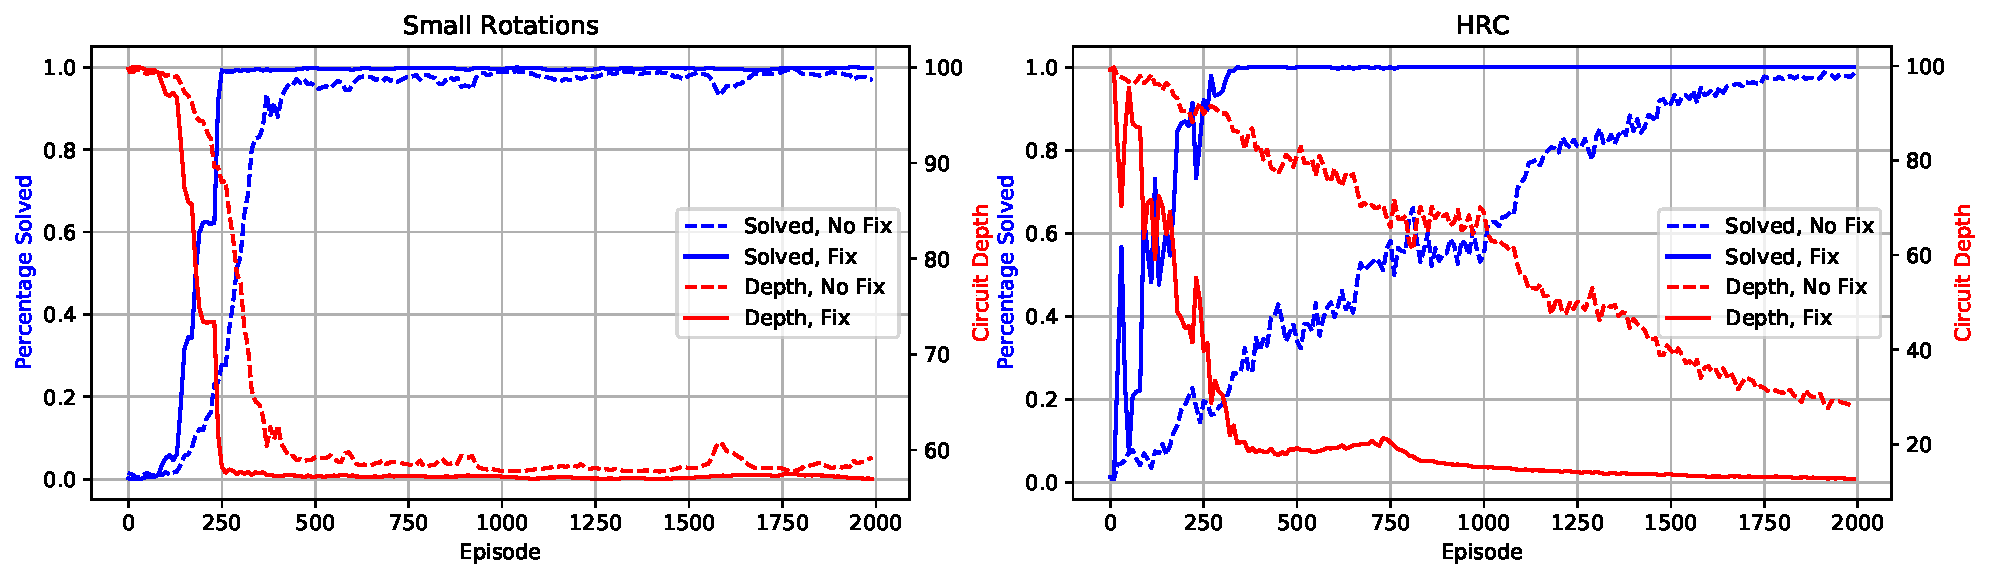
\includegraphics[width=1\textwidth]{../figures/one_qubit_fixvsnofix}
\caption{Fraction solved unitaries and average circuit depth during training of agents compiling one-qubit Haar measure random unitary targets. The tolerance used is $1-\delta = 0.99$, both with and without using phase fix Eq. (\ref{eq:phasefix}) to the discrepancy metric $O_n$ (Eq. (\ref{eq:FUMCmetric})). The basis gate sets used are the small rotations set Eq. (\ref{eq:smallrotations1}) and HRC set Eq. (\ref{eq:HRC1}). The hyperparameters of the agents are described in ... . The average gate fidelity Eq. (\ref{eq:AGFfinite}) is calculated during the training period by evaluating the agent on an independent validation set of 1000 unseen random unitaries.} \label{fig:1}
\end{figure*}

From Fig. \ref{fig:1}, we see that introducing the phase fix generally reduce the number of episodes required to train the agent to reach a good performance. This is most obvious for the HRC gate set, where the the number episodes required to reach a solved percentage of above $90\%$ was was reduced by approximately an order of magnitude. This behaviour is expected, as the phase fix removes the symmetry induced by the global phase of the target unitary. By removing the symmetry, the neural policy does not have to learn explicitly that unitaries that differ in a global phase are optimally compiled in the same way. Hence, the complexity of the learning problem is reduced. Also, the training with the phase fix is more stable and less prone to fluctuations.

\subsection{Scaling Relation}

We are also interested in seeing how the circuit depth $N$ of the compiled circuits scale as a function of the tolerance $\delta$ with and without phase fix. In addition, we investigate how switching to the less expensive FISC approach impacts the scaling. The hyper parameters of the agents can be found in ... . The scaling relations were found by training the various agents using the small rotations gate set with a tolerance $\delta = 0.001$. An average circuit depth was then computed for various $\delta \in [0.001, 0.01]$ on 1000 unseen random unitaries.
The resulting data was then fitted to Eq. \ref{eq:scaling_relation}, which can be seen in Fig. \ref{fig:2}.

\begin{figure*}[h]
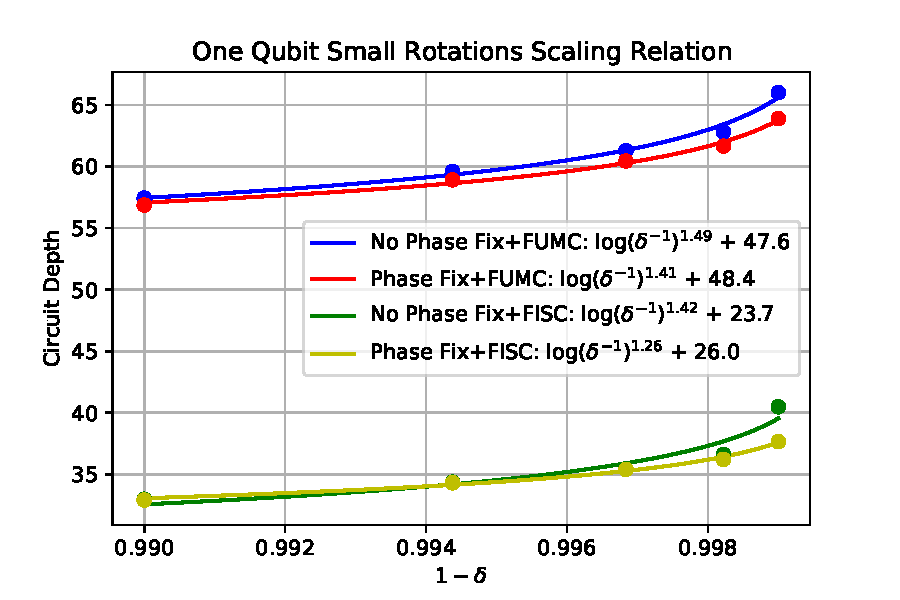
\includegraphics[width=0.7\textwidth]{../figures/one_qubit_scaling}
\caption{Scaling relation between the circuit depth $N$ and tolerance $\delta$ for various agents. The scaling relation was extracted by training the agents to a tolerance of $\delta = 0.001$. An average circuit depth was then computed for various $\delta \in [0.001, 0.01]$ on 1000 unseen random unitaries. The resulting data was then fitted to Eq. (\ref{eq:scaling_relation}).} \label{fig:2}
\end{figure*}

From Fig. \ref{fig:2}, we see that the phase fix results in a favourable scaling relation, with scaling factor $c=1.41$, compared to $c = 1.49$ without phase fix. By reducing the complexity of the problem, the agent is not only able to find good solutions quicker, but is also able to find slightly better solutions with more favorable scaling. Because of this property, we will include the phase fix for the rest of the experiments.

Switching from FUMC to FISC the agent is able to find even shorter sequences, with scaling factor $c=1.20$. This comes of course at the cost of losing the effect of $U_T$ on all but the state $\ket{\boldsymbol{0}}$. However, if we can assume the initial state to be $\ket{\boldsymbol{0}}$ anyway, FISC is to be preferred over FUMC if one wants to minimize the number of gates used.

Note that for quantum compiling with deep learning, the time $t$ required to find the compiled circuit is proportional to the circuit depth, i.e., $t \propto N$. This is because each gate is found with using a forward pass of the neural policy Eq. (\ref{eq:policy}), which can be done in constant time.

\subsection{Curriculum Learning}
In Fig. \ref{fig:3} we attempt to train the agents to compile using the two-qubit HRC set using FISC (and FUMC) with a tolerance of $\delta = 0.95$ ($\delta = 0.75$). The agents are trained using curriculum learning as explained in Sec. \ref{sec:CurriculumLearning}. The target unitaries has an initial depth uniformly sampled as $l \sim U\{1, 2\}$. As the agent is trained, the upper limit is increased by one every $250$ ($2000$) episode to increase the difficulty of the task, up to a maximum of $10$. After $5000$ ($20000$) episodes, the agents are trained for an additional $5000$ ($80000$) episodes using Haar distributed unitaries. The vertical black line indicates this transition. For contrast, we train the other agent for $10000$ ($100000$) episodes using just Haar distributed targets. 

\begin{figure*}[h]
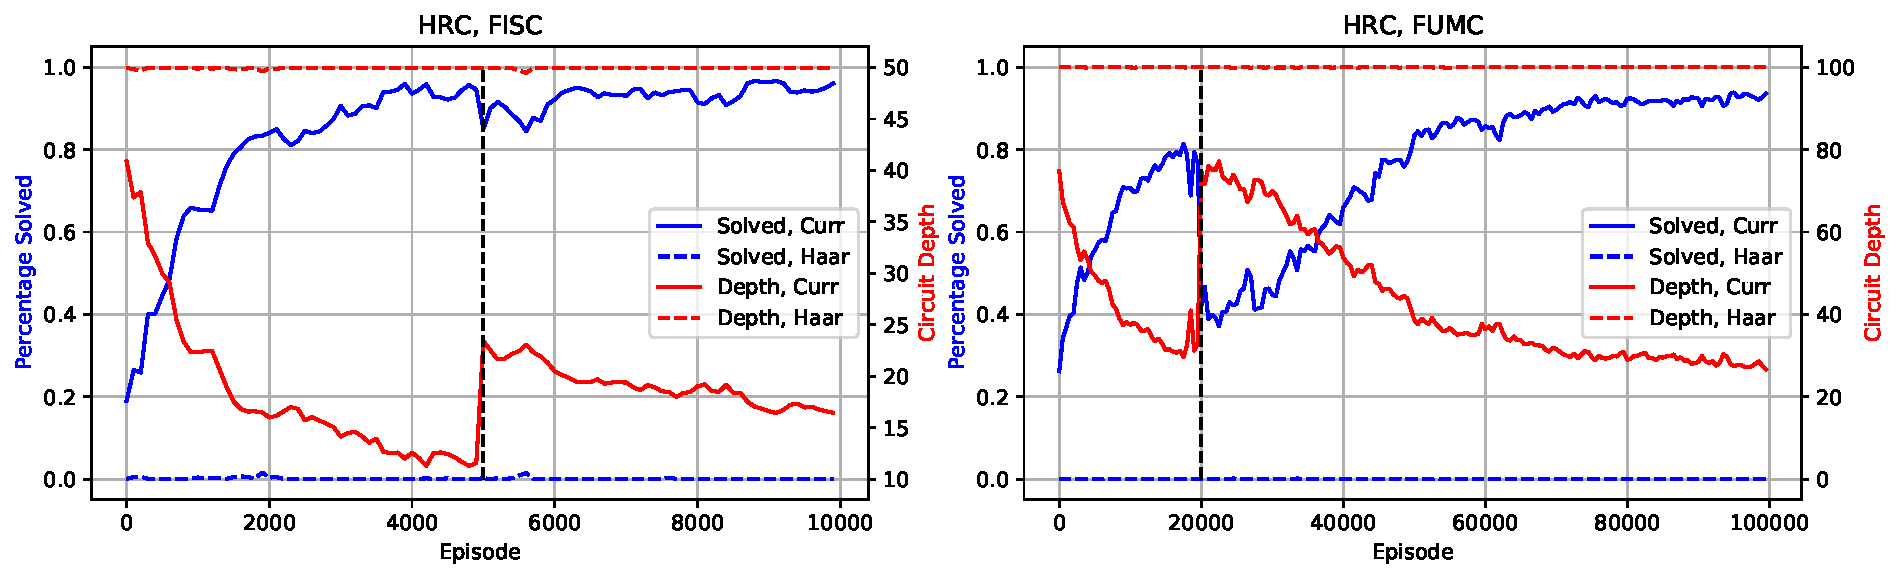
\includegraphics[width=1\textwidth]{../figures/two_qubit_HRC_curriculum}
\caption{Fraction solved unitaries and average circuit depth during training of two agents using the HRC basis set on two qubits. The first agent is trained using curriculum learning (curr) with a max depth of 10 for the first $5000$ episodes, then Haar distributed unitaires for the rest (solid lines). The second agent is trained using just Haar distributed unitaires (dashed lines). The vertical green line (at 5000 episodes) marks when the first agents switches from curriculum learning to Haar. FISC and FUMC is used with a tolerance of $\delta = 0.95$ and $\delta = 0.75$, respectivly. In both cases phase fix of $O_n$ is used. The hyperparameters of the agents are described in ... .} \label{fig:3}
\end{figure*}

From Fig. \ref{fig:3} we see that the agents training on just the two-qubit Haar distribution has problems learning anything at all in the beginning, as opposed to one-qubit Haar distibtion used in Fig. \ref{fig:1}. This is because the Haar distribution containing all possible two qubit unitaries is too difficult to compile for an untrained agent. This leads to mostly failed attempts, from which the agent gains very little information using the sparse reward function. Unlike the dense reward function, the sparse reward function does not give any guiding information to the agent for failed attempts.

Using curriculum learning, the untrained agents are able to solve some of the targets right away since many of them can essentially be solved by performing a few random actions. Thus, the agents receive an informative reward signal right away, even with the sparse reward. By slowly increasing the depth of the target unitaries, the agents slowly learn to compile more and more complicated unitaries. At the 5000 and 20000 episodes mark (for FISC and FUMC, respectivly), both the targets and validation unitaries used are switched for Haar distributed unitaries. Likewise, we see an instantaneous drop in solved percentage to respectively $\sim 90\%$ and $\sim 40 \%$. This shows that curriculum training using short circuits leads to agents that generalize well to Haar distributed unitaries for FISC, and generalizes to some degree for FUMC. Note that the circuit depth also increase when switching to the Haar distribution, since they are more demanding to compile.

Since the pre-training using curriculum learning lets the agents generalize to the Haar distribution, further training on these new targets quickly lets the agents increase their performance. This is in contrast to the agents that train only using the Haar distribution, which ended up learning nothing because of the hardness of the problem. It therefore seems necessary to use curriculum learning for anything beyond one qubit when sparse reward functions are involved. 


Note that we were only able to solve $\sim 95\%$ of target Haar unitaries within a tolerance of $\delta = 0.75$, as seen from Fig. \ref{fig:3}. This is not a particularly high tolerance, and would contribute a large inaccuracy if used to compile quantum algorithms used for practical purposes. However, we believe that this is not a fundamental problem of the deep reinforcement learning based compiling, but rather the specifics of this implementations. Espesially, deep Q-learning is known to very sensitive to hyper-parameters and struggle to converge to optimal policies when faced with large possibility spaces (kilde). It is probable that more sophisticated architectures, like actor-critic models (kilde) will exhibit better generalization and faster convergence when trained to compile.

%However, it does not  This shows that the agent is able to generalize well to Haar distributed unitaries within a tolerance $\delta = 0.05$ by training only on unitaries constructed from a low number of elementary gates. For a depth of $d=10$ using the HRC basis set for two qubits, there is a total of $\sum_{i=1}^{10} 8^i \approx 1.2 \times 10^{9}$ unique sequences. By the end of the first 5000 episodes, we see from Fig. \ref{fig:3} that the agent is able to solve about $95\%$ of these after having seen less than  $N_{max}N_{episodes} = 50\times 5000 = 2.5 \times 10^{5}$ unique sequences. This highlights the powerful generalization of deep reinforcements learning. Of course, the the learning problem was greatly simplified by utilizing FISC with a high tolerance $\delta = 0.05$.  


\section{Conclusion and Future Work \label{sec:6}}
A shortcoming of the discrepancy metrics $O_n = U_T^{\dagger}U_n$ and $O_n = \bra{\boldsymbol{0}}U_T^{\dagger}U_n$ is that the number of elements they represent scales exponentially with the number of qubits. Since they serve as features that are fed to the initial layer of the neural policy, this means that also the number of parameters of the network scales exponentially. This will lead to computationally intractable networks as the number of qubits are increased. Alternatively, one can attempt to learn an approximate discrepancy metric with a polynomial number of elements: 
\begin{equation}
    \Tilde{O}_n = NN(S;\boldsymbol{\Tilde{\theta}}),
\end{equation} 
where $NN$ is a neural network and $S$ is a vector describing the sequence of gates that $O_n = U_T^{\dagger}U_n$ constitute. $S$ is essentially a sparse representation of $O_n$, and $\Tilde{O}_n$ is an embedding of $S$ parameterized by $\boldsymbol{\Tilde{\theta}}$, possibly similar to word-embedding(kilde). This "gate-embedding" would lack the perfect information encoding the difference between $U_T$ and $U_n$. However, if it could still encode enough information for efficient compiling, it would perhaps pave way for deep learning based quantum compilers for a higher number of qubits.



\begin{acknowledgments}
Acknowledgements
\end{acknowledgments}

\section*{Data Availability}
All code, documentation, experiments and results are readily available in following GitHub repository:
https://github.com/KristianWold/QuantumCompiling
%\cite{X1,X2,X3,X4,X5,X6,X7,X8,X9,X10,X11,X12,X13,X14,X15,X17,X18,X19}
%\cite{X21,X22}
% Create the reference section using BibTeX:
\section*{References}
\bibliography{main}

\section*{Appendix}

\begin{table}[h]
\caption{Hyper-parameters of the agents used to produce the results in the left (right) subplot of Fig. \ref{fig:1}.}
\label{tab:tab1}

\begin{tabular}{|l|l|}
\hline
Gate Set & \pbox{20cm}{One-Qubit Small Rot \\ (HRC)}\\ \hline
Target Unitaires & Haar Measure\\ \hline
Reward & \pbox{20cm}{Dense Reward \\ \Sparse Reward)} \\ \hline
Episodes & 2000\\ \hline
Tolerance & $\delta = 0.01$ \\ \hline
Max Depth & $N_{max}=100$ \\ \hline
Memory Capacity & $10^4$ \\ \hline
Batch Size & 1024  \\ \hline
Learning rate & $\lambda = 10^{-5}$ ($\lambda = 10^{-4}$)  \\ \hline
Layers & [256, 128]  \\ \hline
\end{tabular}
\end{table}

\begin{table}[h]
\caption{Hyper-parameters of the agents used to produce the results of Fig. \ref{fig:2}.}
\label{tab:tab2}

\begin{tabular}{|l|l|}
\hline
Gate Set & One-Qubit Small Rot\\ \hline
Target Unitaires & Haar Measure\\ \hline
Reward & Dense Reward \\ \hline
Episodes & \pbox{20cm}{3000 \\ (7300 for FUMC + No Fix)}\\ \hline
Tolerance & $\delta = 0.001$ \\ \hline
Max Depth & $N_{max}=150$ \\ \hline
Memory Capacity & $10^5$ \\ \hline
Batch Size & 2048  \\ \hline
Learning rate & $\lambda = 10^{-5}$  \\ \hline
Layers & [256, 128, 64]  \\ \hline
\end{tabular}
\end{table}

\begin{table}[h]
\caption{Hyper-parameters of the agents used to produce the results of Fig. \ref{fig:3}.}
\label{tab:tab2}

\begin{tabular}{|l|l|}
\hline
Gate Set & Two-Qubit HRC\\ \hline
Target Unitaires & \pbox{20cm}{Curriculum \\ (Haar Measure)}\\ \hline
Reward & Sparse Reward \\ \hline
Episodes & $10^{4}$\\ \hline
Tolerance & $\delta = 0.05$ \\ \hline
Max Depth & $N_{max}=50$ \\ \hline
Memory Capacity & $10^4$ \\ \hline
Batch Size & 2048  \\ \hline
Learning rate & $\lambda = 10^{-5}$  \\ \hline
Layers & [1024, 512, 256, 128]  \\ \hline
\end{tabular}
\end{table}



\end{document}
%
% ****** End of file aiptemplate.tex ******